\section{Entwurf (Daniel)}\label{sec:entwurf}


\subsection{Architektur}
Wie bereits in der Einleitung erwähnt sind die meisten der verwendeten Technologien bereits festgelet.

Da das Ziel dieses Programmentwurfs eine Mobile Applikation ist, ergeben sich aus der Anforderung React zu nutzen folgende Möglichkeiten:
\begin{itemize}
    \item (Progressive) Web App mittles React (Web)
    \item Hybride, native App mit React (Web) und PhoneGap
    \item Hybride, native App mit React Native
\end{itemize}

Aus diesen drei Alternativen ist React Native am nächsten an einer nativen Anwendung.
Im Gegensatz zu PhoneGap wird kein Webview in einer nativen Anwendung genutzt um eine Webapp darzustellen,
sonder es werden tatsächliche native UI-Elemente verwendet.
Dadurch fühlt sich die Anwendung nativer an.


\subsection{Oberflächengestaltung}
Die Gestaltung der Oberflächen orientiert sich an den \textit{Material Design}-Richtlinien von Google.
Auf \cite{DesignMa49:online} werden Richtlinien und Konzepte vorgegeben,
welche Entscheidungen bei der Oberflächengestaltung übernehmen.
Die zudem vorhandene Übersicht an Komponenten lässt sich nutzen um passende Komponenten für einen Anwendungsfall zu finden.

Um erste Ideen für die Oberflächengestaltung zu sammeln,
werden mit Hilfe von dem Tool \textit{Fluid UI} \cite{FluidUIc8:online} sogenannte UI-Mockups erstellt.
Diese Mockups dienen als beispielhafte Vorlage für die spätere Entwicklung.


\begin{figure}[h]
    \centering
    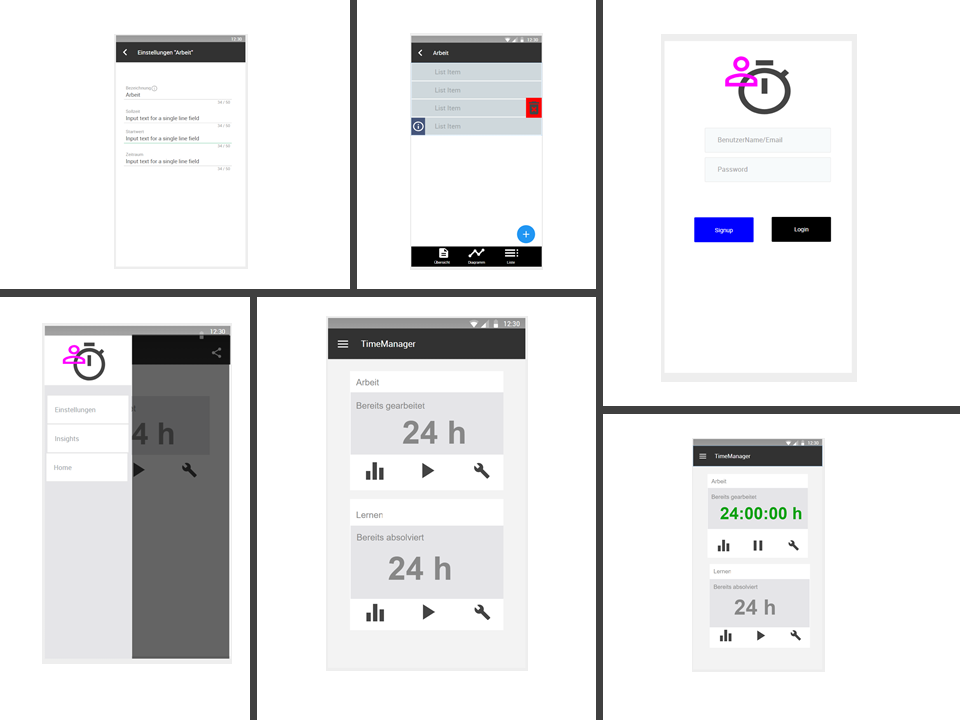
\includegraphics[width=\textwidth]{uiMocks/Mock}
    \caption{UI-Mockups der Anwendung}
\end{figure}



